\chapter{Метод опорных векторов}
\section*{Введение}
В данном разделе рассмотрены основные понятия метода опорных векторов и алгоритм его работы. 
Определения терминов, используемых в данной работе.
\begin{enumerate}
	\item Гиперплоскость – это $(n-1)$-мерная подплоскость в $n$-мерном евклидовом пространстве, которая разделяет пространство на две отдельные части \cite{hyperploskostb}.
	\item Ядро – это функция, которая вычисляет точечное произведение двух векторов в высокоразмерном пространстве \cite{kernel}.
	\item Радиальные базисные функции – это класс функций, которые используются в нейронных сетях для аппроксимации и интерполяции данных \cite{rbf}.
\end{enumerate}

\section*{Основная часть}

Метод опорных векторов – линейный алгоритм, который используется в задачах классификации и регрессии. 
Суть алгоритма – найти линию или гиперплоскость, разделяющую данные на классы.

Изначально метод опорных векторов работает как линейный классификатор, способный решать только задачи, где классы данных можно разделить прямой линией. 
Однако при использовании нелинейных ядер, метод опорных векторов способен преобразовывать исходные данные в пространство более высокой размерности, где можно найти оптимальную разделяющую гиперплоскость \cite{all}. 
Некоторые из популярных ядер метода опорных векторов:
\begin{itemize}
	\item линейное ядро (преобразует данные в ту же размерность без изменений);
	\item полиномиальное ядро (преобразует данные в более высокую размерность с использованием полиномиальной функции);
	\item радиальное базисное функциональное ядро (преобразует данные в бесконечно высокую размерность с использованием радиальной базисной функции).
\end{itemize}

Пример. На рисунке \ref{pic_1} изображен набор данных, который необходимо классифицировать и отделить квадраты от треугольников. Существует бесконечное количество линий, способных разделить эти два класса. Основная цель в поставленной задаче – найти оптимальную из них.

\begin{figure} [H]
	\centering{
		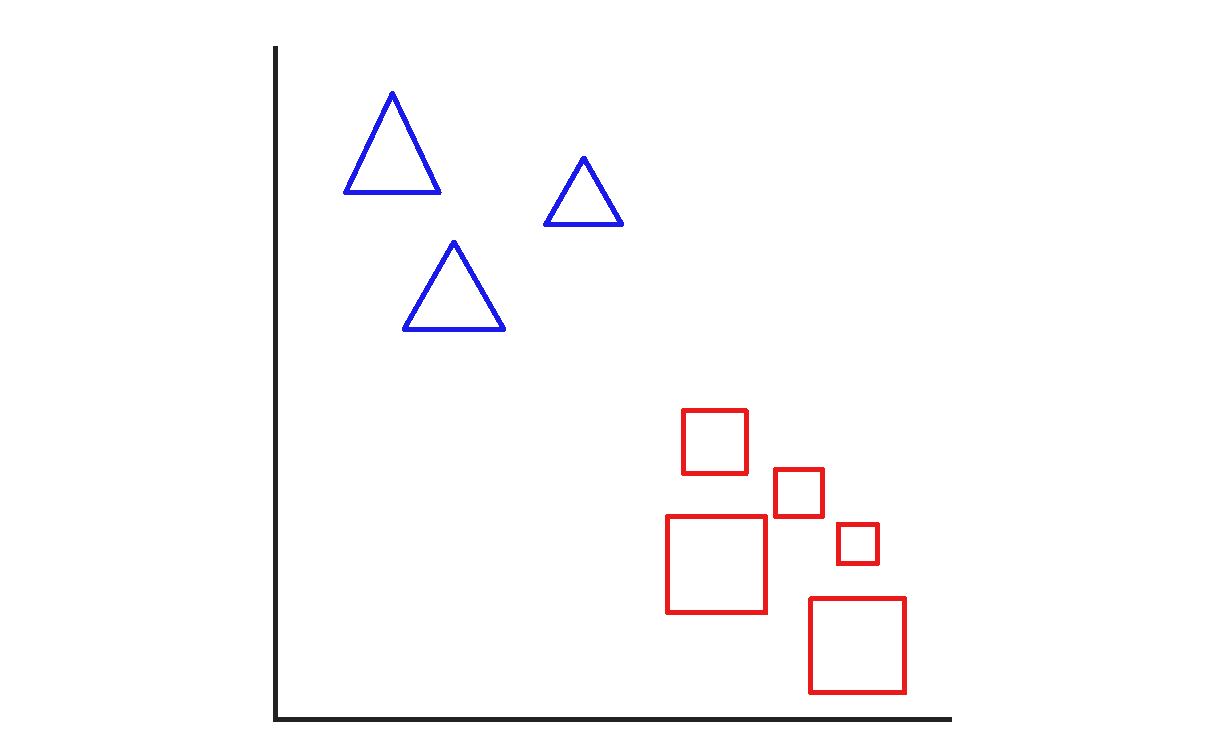
\includegraphics[scale=0.7]{img/circles.pdf}
		\caption{Исходные данные}
		\label{pic_1}
	}
\end{figure}

На рисунке \ref{pic_2} изображены два варианта разделения на классы.

\begin{figure} [H]
	\centering{
		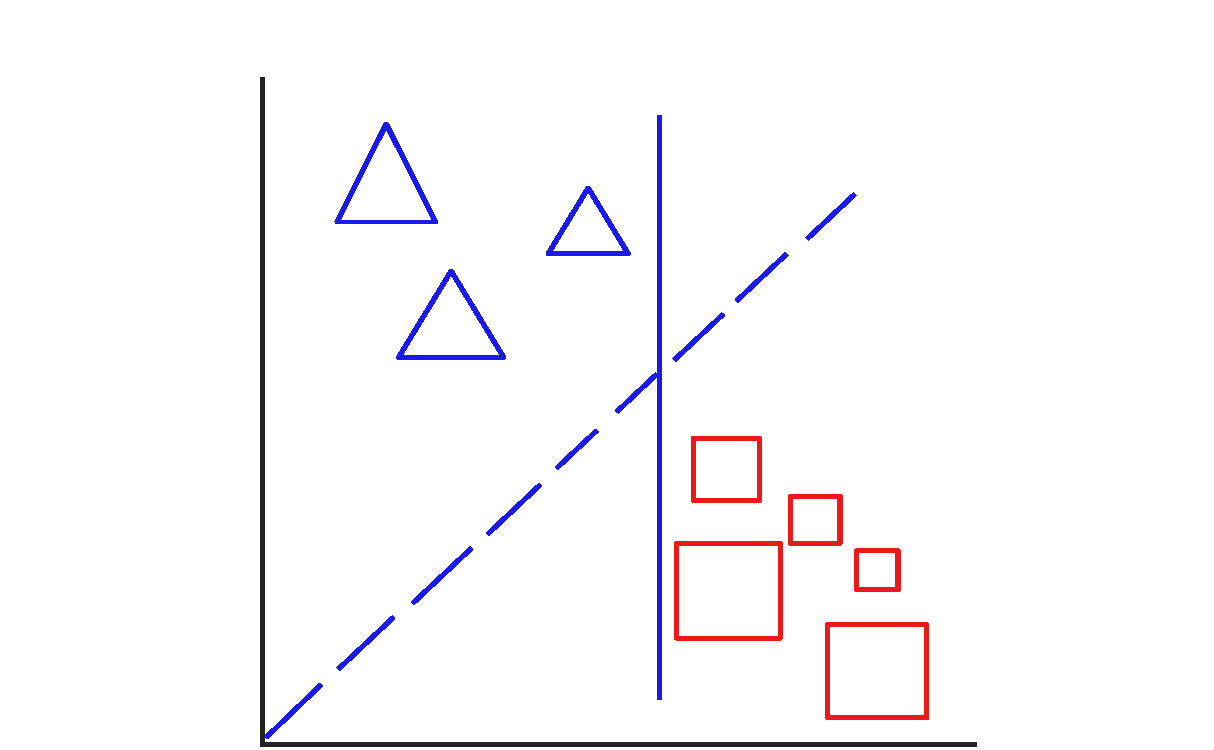
\includegraphics[scale=0.7]{img/circles2.pdf}
		\caption{Варианты разделяющих линий}
		\label{pic_2}
	}
\end{figure}

Сплошная линия проходит слишком близко к классам треугольников и квадратов. Несмотря на то, что она верно классифицировала все объекты текущего набора данных, она не будет генерализованной, не будет так же хорошо разграничивать незнакомый набор данных. Поэтому в данном случае оптимальные выбор -- прерывистая линия \cite{all}.

Основные этапы метода опорных векторов.
\begin{enumerate}
	\item Подготовка обучающего набора данных, состоящего из пар (вектор признаков, метка класса).
	\item Выбор ядра и настройка параметров модели.
	\item Минимизация функции потерь с использованием оптимизационных методов для нахождения гиперплоскости, максимально разделяющей классы.
	\item Нахождение опорных векторов (опорные векторы -- точки данных, лежащие на границах зазора между классами).
	\item Определение гиперплоскости: гиперплоскость строится для максимизации зазора между классами с учетом опорных векторов и параметров ядра.
	\item Оценка обобщающей способности модели на тестовой выборке для проверки ее работоспособности на новых данных.
\end{enumerate}
